% Portada del tema «Bases covariantes y contravariantes» (ilustrativa, geometría exacta).
% Base oblicua a 60°:  g1 = (1,0), g2 = (1/2, √3/2);  recíproca  g^1 = (1,−1/√3), g^2 = (0, 2/√3).
% Vector V = (2, 3/2) con V^1 = 2−(3/2)/√3, V^2 = 3/√3  y  V_1 = V·g1 = 2, V_2 = V·g2 = 1+3√3/4.
% Los valores se comprueban en julia/test/runtests.jl («Base oblicua a 60°»).
% Compilar con: scripts/compilar_tikz.sh   (→ figures/svg/portada-bases.svg)
\def\pgfsysdriver{pgfsys-dvisvgm.def}
\documentclass[tikz,border=0pt]{standalone}
\usetikzlibrary{calc,arrows.meta}
% PALETA-INICIO (generado por scripts/sincronizar_paleta.jl; no editar a mano)
\definecolor{azul}{HTML}{1B6CA8}
\definecolor{naranja}{HTML}{D95F02}
\definecolor{verde}{HTML}{2A9D8F}
\definecolor{gris}{HTML}{6B7280}
\definecolor{violeta}{HTML}{6F42C1}
\definecolor{ocre}{HTML}{8A5A00}
\definecolor{malla}{HTML}{CBD5E1}
% PALETA-FIN
\begin{document}
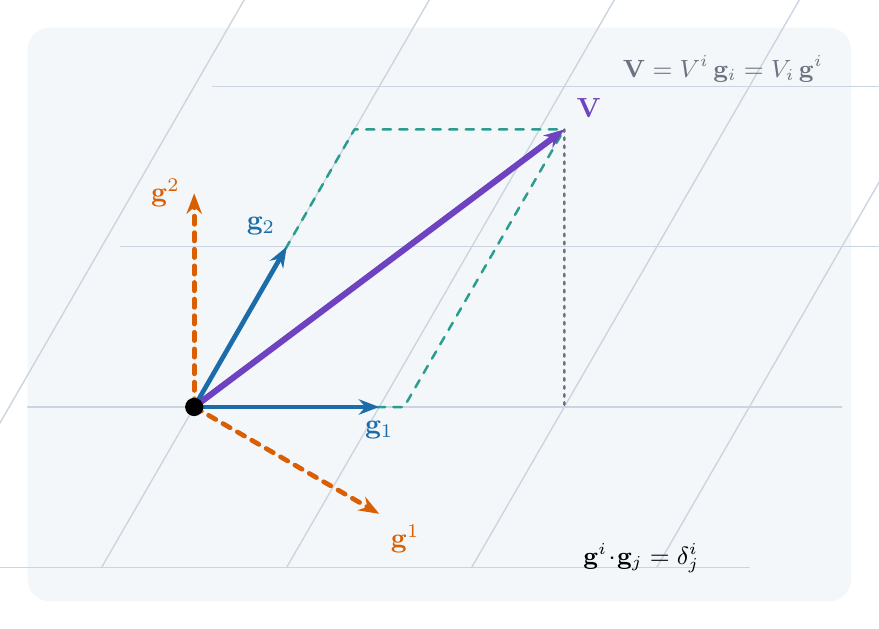
\begin{tikzpicture}[scale=2.35, line cap=round, line join=round, >={Stealth[length=2.6mm]}]
  \pgfmathsetmacro{\rt}{sqrt(3)}
  \useasboundingbox (-0.9,-1.05) rectangle (3.55,2.05);
  \fill[rounded corners=8pt, fill={rgb,255:red,244;green,247;blue,250}] (-0.9,-1.05) rectangle (3.55,2.05);
  % Rejilla de coordenadas oblicuas
  \foreach \k in {-1,0,...,3}{
    \draw[malla, line width=0.5pt] ({\k+(-1)*0.5},{(-1)*\rt/2}) -- ({\k+3*0.5},{3*\rt/2});
  }
  \foreach \k in {-1,0,...,2}{
    \draw[malla, line width=0.5pt] ({\k*0.5-0.9},{\k*\rt/2}) -- ({\k*0.5+3.5},{\k*\rt/2});
  }
  % Construcción de V: V^1 g1 + V^2 g2 (componer) y proyecciones (V_1, V_2)
  \coordinate (O) at (0,0);
  \coordinate (V) at (2,1.5);
  \pgfmathsetmacro{\vuno}{2-1.5/\rt}
  \pgfmathsetmacro{\vdos}{3/\rt}
  \draw[verde, dashed, line width=0.9pt] (O) -- (\vuno,0) -- (V);
  \draw[verde, dashed, line width=0.9pt] (O) -- ({\vdos*0.5},{\vdos*\rt/2}) -- (V);
  \draw[gris, dotted, line width=0.9pt] (V) -- (2,0);
  % Bases
  \draw[azul, ->, line width=1.7pt] (O) -- (1,0) node[below=1pt] {$\mathbf{g}_1$};
  \draw[azul, ->, line width=1.7pt] (O) -- (0.5,{\rt/2}) node[above left=0pt] {$\mathbf{g}_2$};
  \draw[naranja, ->, dashed, line width=1.7pt] (O) -- (1,{-1/\rt}) node[below right=0pt] {$\mathbf{g}^1$};
  \draw[naranja, ->, dashed, line width=1.7pt] (O) -- (0,{2/\rt}) node[left=1pt] {$\mathbf{g}^2$};
  \draw[violeta, ->, line width=2.2pt] (O) -- (V) node[above right=0pt] {$\mathbf{V}$};
  \fill (O) circle (1.4pt);
  % Rótulo
  \node[anchor=south west, font=\small] at (2.05,-0.95) {$\mathbf{g}^i\!\cdot\!\mathbf{g}_j=\delta^i_j$};
  \node[anchor=north east, font=\small, text=gris] at (3.45,1.95) {$\mathbf{V}=V^i\,\mathbf{g}_i=V_i\,\mathbf{g}^i$};
\end{tikzpicture}
\end{document}
